% =============================================================
% 面向云–边 LLM 推理调度的 Pareto 占优强化学习方法
% 中文版（基于英文 IEEEtran 双栏，xeCJK 渲染中文）
%
% 编译：make  (使用 xelatex + bibtex + 2x xelatex)
% =============================================================

\documentclass[conference]{IEEEtran}

% --- 中文支持（ctex + xeCJK，IEEEtran 双栏不变） -----------------
\usepackage[UTF8,fontset=macnew]{ctex}
% macnew 选 PingFang/Songti 系列；其他系统也可换 fontset=adobe / windows / ubuntu

% --- 通用宏包 --------------------------------------------------
\usepackage{amsmath,amssymb,amsfonts}
\usepackage{graphicx}
\usepackage{booktabs}
\usepackage{array}
\usepackage{xcolor}
\usepackage{hyperref}
\usepackage{cite}
\usepackage{url}
\usepackage{textcomp}

% --- 图片路径 ---------------------------------------------------
\graphicspath{{figures/}}

% --- hyperref 样式 ---------------------------------------------
\hypersetup{
  colorlinks = true,
  linkcolor  = black,
  citecolor  = blue!50!black,
  urlcolor   = blue!50!black,
}

% --- 常用宏 ----------------------------------------------------
\newcommand{\slo}{SLO}
\newcommand{\etok}{$E$/tok}

% --- 中英混排时给 LaTeX 更多换行灵活度，减少超宽溢出 ---------
\sloppy
\emergencystretch=3em

% --- 标题与作者 ------------------------------------------------
\title{面向云--边 LLM 推理调度的 Pareto 占优强化学习方法}

\author{
  \IEEEauthorblockN{匿名作者}
  \IEEEauthorblockA{送审单位匿名\\
                    邮箱：anonymous@example.com}
}

\begin{document}

\maketitle

% =============================================================
% =============================================================
% 中英文摘要（中文期刊惯例：双语并存）
% =============================================================

\begin{abstract}
\textbf{中文摘要。}大语言模型（LLM）推理负载的快速增长带来了服务成本与能耗压力，单轴吞吐量导向的调度器已无法应对。本文研究 AI 生成内容（AIGC）服务特有的五项物理约束下的\emph{云--边 LLM 推理调度}：模型权重驻留、键值（KV）缓存本地性、连续批处理、解码阶段的显存带宽下限，以及两阶段请求生命周期。我们设计了一个 AIGC 感知的近端策略优化（PPO）调度器，通过状态特征与奖励整形将上述物理量显式暴露给策略网络，并与涵盖启发式、负载均衡、bandit、多目标搜索与学习式方法的 10 个基线对比。在覆盖拓扑、负载与工作负载组合的 30 种配置（每种 $N{=}30$ 次运行）下，本文调度器于典型工况在均值性能上取得严格 Pareto 占优：相对最强单目标基线，服务等级目标（\slo{}）达成率提升 28\%（统计显著，$p<0.05$），同时每 token 能耗降低 7\%。即便面对总体最强基线---膝点 NSGA-II 搜索---本文调度器在两项均值指标上仍更优，且在中等负载下差异显著（$p<0.01$），在每一种配置下每 token 能耗都更低，而调度时计算开销少 $5\times$。然而，12 组件消融揭示联合增益是一项系统级整体贡献：仅连续批处理仿真与充足预训练个体显著；所有 AIGC 奖励与状态组件在单独消融时均与完整模型在统计上不可区分。我们开源仿真器及 30+ 套基准 manifest，以支持后续 AIGC 调度研究。

\textbf{关键词：}LLM 推理；AIGC；云边协同；强化学习；调度；能效；Pareto 优化。

\textbf{中图分类号：}TP18

\textbf{文献标识码：}A
\end{abstract}

% --- English Abstract（中文期刊要求双语并存） -----------------
\noindent\textbf{Abstract.} The rapid growth of large language
model (LLM) inference workloads
imposes serving-cost and energy pressures that single-axis
throughput-oriented schedulers cannot address. We study
\emph{cloud-edge LLM inference scheduling} under five
physical constraints specific to AI-generated-content (AIGC)
serving: model-weight residency,
key-value (KV) cache locality, continuous batching, the
memory-bandwidth floor of decode, and the two-phase
request lifecycle. We design an AIGC-aware
proximal policy optimization (PPO) scheduler that exposes these
physics to the policy through state features and reward
shaping, and compare it against ten baselines spanning
heuristic, load-balancing, bandit, multi-objective search,
and learned approaches.
Across 30 configurations sweeping topology, load, and workload
composition ($N{=}30$ runs each), our scheduler achieves
strict Pareto dominance on mean performance in the canonical
operating regime: a
28\% gain in service-level-objective (\slo) attainment
(statistically significant,
$p<0.05$) together with 7\% lower energy per token relative to
the strongest single-objective baseline. Even against a
knee-point NSGA-II search---the strongest baseline
overall---our scheduler is better on both means,
significantly so at moderate load ($p<0.01$), with lower
energy per token in every configuration at $5\times$ less
scheduling-time compute. A 12-component ablation,
however, reveals that the joint gain is a holistic system
contribution: only continuous-batching simulation and adequate
pretraining are individually significant; every AIGC reward and
state component is statistically indistinguishable from the full
model when ablated alone. We release the simulator and the 30+
benchmark manifests to support future AIGC scheduling research.

\noindent\textbf{Key words:} LLM inference; AIGC; cloud-edge
computing; reinforcement learning; scheduling; energy
efficiency; Pareto optimization.


\begin{IEEEkeywords}
LLM 推理；AIGC；云边协同；强化学习；调度；能效；Pareto 优化。
\end{IEEEkeywords}

% =============================================================
% =============================================================
% §1 引言
% =============================================================
\section{引言}
\label{sec:intro}

以大语言模型（LLM）推理为主导的生成式 AI 负载---亦称 AI 生成内容（AIGC）负载---已成为现代数据中心增长最快的算力类目：其能耗成本在五年间增长了数个数量级~\cite{patterson2021carbon}，且推理消耗的累计 FLOPs 已超过训练~\cite{patel2024splitwise}。随着 LLM 服务进入延迟敏感应用，系统社区正在重新思考推理负载应如何在异构算力资源池上\emph{调度}。

本文研究\textbf{云--边协同 LLM 推理调度}。该部署范式因三点原因日益受到关注：（i）\textbf{成本}---常见请求由更便宜的边缘加速器服务，云端 GPU 留给尾部请求；（ii）\textbf{隐私}---尽可能将 prompt 数据保留在本地；（iii）\textbf{尾延迟}---借助边缘临近性摊薄首 token 延迟。这里的\emph{协同}指部署层面的协作---云与边两层共同服务同一负载---而非多智能体决策：本文研究的每个调度器均为单一集中式策略。我们的优化目标（\S\ref{sec:sched-problem}）直接刻画尾延迟与成本：前者经由服务等级目标（\slo{}）达成率，后者经由每 token 能耗---最主要的边际服务成本；隐私是\emph{部署}云边资源池的动机，但与逐请求放置正交（可编码为可行性掩码，\S\ref{sec:mdp}，留作未来工作）。调度问题---决定每个请求应由哪台服务器服务---由此成为关键性能杠杆，且区别于 vLLM~\cite{kwon2023vllm}、Orca~\cite{yu2022orca}、Sarathi-Serve~\cite{agrawal2024sarathi} 等服务器内部批处理引擎。

\subsection{LLM 推理调度的特殊性}

现有集群调度器---异构最早完成时间（Heterogeneous Earliest Finish Time, HEFT）等表调度启发式、遗传算法（GA）与粒子群优化（PSO）等元启发式，以及 Decima~\cite{mao2019decima}、RLScheduler~\cite{zhang2020rlscheduler} 等学习式变体---原本为 Spark 作业、高性能计算（HPC）批任务等通用有向无环图（DAG）负载设计。它们并未建模从根本上区分 LLM 推理的五项物理特性：

\begin{enumerate}
\item \textbf{模型权重驻留。}LLM 权重（LLaMA-7B/13B/70B~\cite{touvron2023llama} 为 14--70~GB）持久驻留于 GPU 显存；切换模型需付出 5--60~s 的冷加载~\cite{fu2024serverlessllm}---比任何单请求计算高出数个数量级。

\item \textbf{KV cache 本地性。}每个请求的键值（KV）缓存与运行 prefill 的 GPU 绑定；迁移它需为每个请求移动数百 MB 数据，时常主导 decode 延迟~\cite{patel2024splitwise,kwon2023vllm}。

\item \textbf{连续批处理。}迭代级批处理以 ${\approx}(1 + (N-1)\alpha)\,T_{\text{solo}}$ 的时间服务 $N$ 个同模型请求---带来 $5$--$8\times$ 吞吐增益~\cite{yu2022orca,kwon2023vllm}，但只有当调度器将同模型请求共置时才能兑现。

\item \textbf{显存带宽受限的 decode。}与计算受限的 prefill 不同，decode 受高带宽显存（HBM）带宽约束：A100 级 GPU 上每 token ${\approx}20$~ms~\cite{patel2024splitwise,agrawal2024sarathi}，与算力无关。

\item \textbf{两阶段请求生命周期。}每个请求分解为 Prefill$\,\to\,$Decode，二者具有严格依赖与共享 KV 状态~\cite{zhong2024distserve}，违反了大多数 DAG 调度器的"各阶段独立"假设。
\end{enumerate}

这五项物理特性带来了通用负载所没有的权衡：集中同模型请求（利于批处理）还是分散它们（避免争用）；将 decode 派往快但远的服务器，还是派往其兄弟 prefill 服务器（免去 KV 迁移）。\textbf{忽略 AIGC 物理的调度器无法利用这些权衡}。

\subsection{为什么朴素方法会失效}

一个自然的猜想是：现成的强化学习（RL）调度器可以从基础特征（算力、队列长度、显存）中\emph{隐式}学到 AIGC 感知行为。我们正是为检验这一猜想而开展本工作；实证图景更为微妙（图~\ref{fig:pareto}）：

\begin{itemize}
\item 通用负载均衡基线（LeastLoaded、ShortestQueue）、最优 DAG 启发式（HEFT、GA、PSO）、PerLLM 风格的受限 bandit 调度器~\cite{yang2024perllm}，乃至现代深度强化学习（DRL）基线（A3C-R2N2~\cite{tuli2022a3cr2n} 与我们自实现的 Decima 风格图神经网络（GNN）变体~\cite{mao2019decima}）全部聚集在同一 Pareto 区域：\slo{} 达成率约 19--24\%，能效约 2.8--3.0 J/token。

\item 我们的 AIGC 感知近端策略优化（PPO）调度器与 A3C-R2N2 共用 actor-critic 家族与等价预训练预算，但加入显式 AIGC 状态特征与奖励整形，取得\textbf{明显更优的 Pareto 点}：\slo{} 30.2\%（相对 $+28\%$）、能耗 2.61~J/token（相对 $-7\%$），\slo{} 维度对全部 5 个最强单目标基线均 $p<0.05$。总体最强基线---我们同样实现的膝点 NSGA-II 搜索---在典型工况点接近本文的 \slo{}，但在中等负载下被显著超越（$p<0.01$），在每一种配置下付出更多能耗，且派发时计算开销高 $5\times$。

\item 然而，我们的 12 组件消融（表~\ref{tab:ablation}、图~\ref{fig:ablation}）揭示了一个悖论：移除任何单一 AIGC 组件（warm 奖励、batch 奖励、affinity 奖励、AIGC 状态特征，甚至全部联合移除）后，性能几乎不变。只有连续批处理仿真与充足预训练凸显为显著组件。
\end{itemize}

\subsection{调和与贡献}

认识到\textbf{AIGC 感知调度是一项系统级整体贡献，而非某个巧妙的奖励组件}，上述观察即可得到调和。一旦调度器具备（i）环境中的连续批处理物理、（ii）充足的预训练、（iii）状态或奖励中某种形式的 AIGC 感知，PPO 主干便能从任一 AIGC 先验中提取等价信号---它们可互相替代。Pareto 改进是真实的，但它来自\emph{组合}，而非单个奖励技巧。

\smallskip
\noindent 本文做出四项贡献：

\noindent\textbf{（C1）AIGC 推理仿真平台}，建模全部五项物理特性：带最近最少使用（LRU）驱逐的权重驻留、带 KV cache 显存核算的 prefill/decode 两阶段任务、准入时连续批处理，以及按 vLLM 实测标定的显存带宽下限。平台随复现 manifest 一并开源。

\noindent\textbf{（C2）AIGC 感知 PPO 调度器（RL）}，通过状态特征（已加载模型指示、批占用率、兄弟服务器亲和、KV cache 体积）与奖励整形（warm、batch、affinity bonus；cloud-overuse 惩罚）将 AIGC 物理暴露给策略网络，在 \slo{} 达成率与能效两个维度对 10 个强基线取得\textbf{均值性能上的 Pareto 占优}。

\noindent\textbf{（C3）系统性的 12 组件消融研究}，揭示哪些 AIGC 抽象真正有贡献。醒目的零结果---没有任何单项 AIGC 奖励或状态组件个体显著---警示后续工作：在缺乏联合消融时，不应将增益归因于特定奖励设计。

\noindent\textbf{（C4）实证的"工况"刻画}，表明 AIGC 感知 RL 仅在\textbf{中等负载工况}（$\lambda \in [1, 2]$ 请求/秒、uniform 模型混合）取得严格 Pareto 占优，同时在全部 30 种测试配置下保持最低的每 token 能耗，且相对最强基线的优势随负载增长---这一细致发现与 DRL 调度文献中常见的"处处取胜"论断相悖。

\smallskip
本文其余部分依次介绍背景（\S\ref{sec:background}）、形式化问题（\S\ref{sec:formulation}）、仿真器与调度器设计（\S\ref{sec:system}）、评估（\S\ref{sec:eval}）、讨论（\S\ref{sec:discuss}）、相关工作（\S\ref{sec:related}）与结论（\S\ref{sec:conclusion}）。

% =============================================================
% §2 背景
% =============================================================
\section{背景}
\label{sec:background}

\subsection{LLM 推理：Prefill、Decode 与 KV cache}
\label{sec:bg-inference}

\begin{figure*}[t]
  \centering
  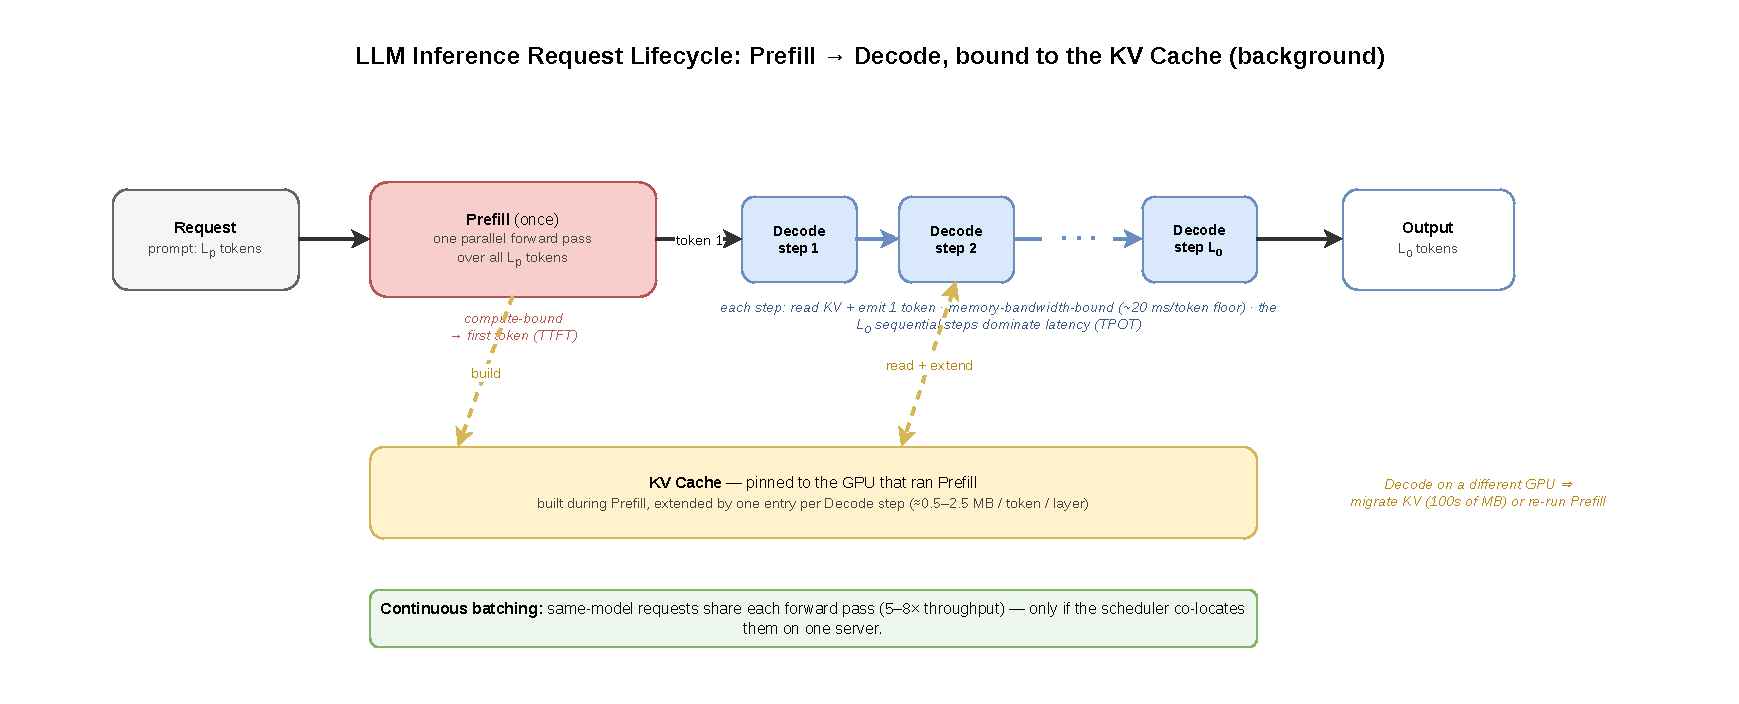
\includegraphics[width=0.70\textwidth]{llm_inference_lifecycle.pdf}
  \caption{一次 LLM 推理请求的两阶段生命周期。\emph{Prefill} 对整段 prompt 执行一次（计算受限），输出首个 token 并建立 KV cache；\emph{Decode} 随后执行 $L_o$ 个串行的、显存带宽受限的步骤，每步读取并追加 KV cache。KV cache 绑定在运行 Prefill 的那台 GPU 上，因此把 Decode 派到别处会强制 KV 迁移或重跑 Prefill——这正是跨服务器调度器必须权衡的核心本地性张力。}
  \label{fig:lifecycle}
\end{figure*}

现代 LLM 是 decoder-only Transformer~\cite{vaswani2017attention,brown2020gpt3}，其推理分为两个硬件特征截然不同的阶段（图~\ref{fig:lifecycle}）。\textbf{Prefill} 每请求执行一次：在一次使算力饱和的前向传播中处理长度为 $L_p$ 的 prompt，产生首个输出 token 及每一层对应的\emph{键值缓存}（KV cache）。\textbf{Decode} 随后迭代执行，每个输出 token 一步（A100 上约 $10$--$80$~ms），复用并追加 KV cache；对长生成场景，$L_o$ 步序列主导端到端延迟。

KV cache 体积大（每 token 每层 $0.5$--$2.5$~MB；1000-token 的 LLaMA-13B 会话约 800~MB）且\textbf{与运行 Prefill 的 GPU 绑定}：在别处服务 Decode 要么通过网络拷贝数百 MB，要么重跑 Prefill。

除 Transformer LLM 之外，AIGC 负载还包括文本生成图像的扩散模型，其推理在每个去噪步都调用同一个共享 U-Net——在结构上与 LLM 不同，但共享同样的模型驻留与批处理特性，这正是本文工作的动机所在。

\subsection{连续批处理与现代服务系统}
\label{sec:bg-batching}

\textbf{连续（迭代级）批处理}——由 Orca~\cite{yu2022orca} 引入、vLLM~\cite{kwon2023vllm}（PagedAttention）与 Sarathi-Serve~\cite{agrawal2024sarathi}（分块 prefill）进一步精炼——在每个 decoder 迭代都重组当前批：完成的请求即时退出，排队请求中途加入。每请求批处理开销在 decode 阶段 $<5\%$（显存带宽受限），在 prefill 阶段约 30\%（算力受限）——即本文仿真器采用的阶段相关系数（\S\ref{sec:simulator}）。这些引擎级优化仅作用于\textbf{单台服务器之内}；\emph{某个请求由哪台服务器处理}这一上游问题正是本文聚焦的对象。

\subsection{云--边协同 LLM 部署}
\label{sec:bg-cloudedge}

生产环境的 LLM 服务越来越多地跨越异构算力池部署：一台或多台云服务器配备高端加速器（A100/H100，GPU 显存即 VRAM $\ge$80~GB），可承载 LLaMA-70B-INT8（约 70~GB）的高吞吐服务；一组边缘服务器涵盖数据中心 A100、工作站级 T4 直至嵌入式 Jetson Orin，显存 16--64~GB、算力 10--50 TFLOPS、热设计功耗（TDP）30--250~W，适合 LLaMA-7B/13B 等较小变体；以及一张云--边往返延迟 30--65~ms、边--边往返延迟 8--23~ms 的网络。该范式由\textbf{延迟}（边缘临近降低首 token 延迟，TTFT）、\textbf{成本}（边缘 GPU 每 FLOP 便宜 1--10$\times$，功耗低 2--10$\times$）与\textbf{数据主权}驱动。阶段解耦与迁移类系统（\S\ref{sec:related}）重新设计部署本身；我们回答它们留下的互补的\emph{初始放置}问题：给定固定的异构池，每个请求应派往何处？

\subsection{调度方法}
\label{sec:bg-sched}

云--边调度历来使用启发式调度器（HEFT~\cite{topcuoglu2002heft}、Round-Robin/Least-Loaded/Shortest-Queue）、元启发式（GA~\cite{holland1975adaptation}、PSO~\cite{kennedy1995pso}）与学习式调度器（Decima~\cite{mao2019decima}、RLScheduler~\cite{zhang2020rlscheduler}，以及拓扑上最接近的 A3C-R2N2~\cite{tuli2022a3cr2n}——面向通用边缘--云任务、采用门控循环单元（GRU）+ 残差编码器的异步优势 actor-critic）。它们均未原生编码 AIGC 物理：启发式将任务视作独立黑盒，元启发式的 fitness 函数需要手工设计 AIGC 项——这正是本文自动化的环节——而现有学习式调度器均早于 LLM 时代。我们在第~\ref{sec:related} 节深入综述这一图景，并在第~\ref{sec:eval} 节对三类方法全部进行基准比较。

% =============================================================
% §3 问题形式化
% =============================================================
\section{问题形式化}
\label{sec:formulation}

本节将云--边 LLM 推理调度问题形式化。\S\ref{sec:sys-model} 引入部署拓扑与负载的符号；\S\ref{sec:physics-constraints} 将五项 AIGC 物理表达为作用于调度决策的约束与代价函数；\S\ref{sec:sched-problem} 将我们的调度问题表述为多目标优化；\S\ref{sec:mdp} 将其转化为 Markov 决策过程（MDP）以便强化学习求解。表~\ref{tab:notation} 汇总了本节通篇使用的符号。

\begin{table}[t]
  \centering
  \caption{\S\ref{sec:formulation} 所用符号。}
  \label{tab:notation}
  \small
  \setlength{\tabcolsep}{4pt}
  \begin{tabular}{@{}l@{\hspace{8pt}}p{0.60\columnwidth}@{}}
    \toprule
    符号 & 含义 \\
    \midrule
    \multicolumn{2}{@{}l}{\emph{拓扑与服务器}} \\
    $\mathcal{S} = \{s_0, \ldots, s_N\}$
      & 服务器池：云 $s_0$，边缘 $s_1, \ldots, s_N$ \\
    $C_s$, $V_s$, $B_s$
      & $s$ 的算力（TFLOPS）、显存（GB）与带宽（Mbps） \\
    $P^{\text{idle}}_s$, $P^{\max}_s$
      & $s$ 的空闲与峰值功耗（W） \\
    $u_s(t)$, $P_s(t)$
      & $s$ 的利用率与瞬时功率 \\
    $\tau(s, s', x)$
      & 从 $s$ 到 $s'$ 传输 $x$~GB 所需时间 \\
    \addlinespace
    \multicolumn{2}{@{}l}{\emph{模型目录}} \\
    $\mathcal{M} = \{m_1, \ldots, m_K\}$
      & LLM 变体目录 \\
    $W_m$, $C^{\text{cold}}_m$
      & $m$ 的权重体积（GB）与冷加载时间（s） \\
    $\kappa_m$, $\phi_m$, $B^{\max}_m$
      & $m$ 的单 token KV 大小、解码下限、最大 batch \\
    $L_s(t)$
      & 时刻 $t$ 已加载到 $s$ 上的模型集合 \\
    \addlinespace
    \multicolumn{2}{@{}l}{\emph{负载}} \\
    $\mathcal{R}$, $\lambda$
      & 请求流与 Poisson 到达率（req/s） \\
    $r_i = (m_i, L^p_i, L^o_i, a_i)$
      & 目标模型、prompt/输出长度、到达时间 \\
    $t^{\text{pre}}_i$, $t^{\text{dec}}_i$
      & 请求 $r_i$ 的 prefill 与 decode 任务 \\
    $w_t$, $n_t$
      & 任务 $t$ 的工作量（TFLOPS）与 token 数 \\
    \addlinespace
    \multicolumn{2}{@{}l}{\emph{执行与目标}} \\
    $\delta^{\text{cold}}$, $\delta^{\text{kv}}$
      & 冷加载与 KV 迁移延迟 \\
    $b_{s,m,k}(t)$, $\beta_k$
      & 批占用；阶段 $k$ 的开销系数 \\
    $T^{\text{solo}}$, $T^{\text{exec}}_{\text{eff}}$
      & 独占 / 批处理执行时间 \\
    $e^{\text{pre}}_i$; $s^{\text{dec}}_i$, $e^{\text{dec}}_i$
      & prefill 完成时刻；decode 开始与完成时刻 \\
    $\text{TTFT}_i$, $\text{TPOT}_i$
      & 首 token 延迟、每输出 token 时间 \\
    $T^*_{\text{TTFT}}$, $T^*_{\text{TPOT}}$
      & TTFT 与 TPOT 的 \slo{} 阈值 \\
    $\text{SLO}(\pi)$, $E_{\text{tok}}(\pi)$
      & 策略 $\pi$ 下的 \slo{} 达成率与每 token 能耗 \\
    $\pi$; $\mathbf{s}_t$, $a_t$, $r_t$
      & 调度策略；MDP 状态、动作、奖励 \\
    \bottomrule
  \end{tabular}
\end{table}

\subsection{系统模型}
\label{sec:sys-model}

\textbf{部署拓扑。}异构算力池 $\mathcal{S} = \{s_0, s_1, \ldots, s_N\}$，其中 $s_0$ 为云服务器，$s_1, \ldots, s_N$ 为边缘服务器。每台服务器 $s$ 具有固定属性：算力 $C_s$（TFLOPS）、显存容量 $V_s$（GB）、上行带宽 $B_s$（Mbps），以及空闲与峰值功耗 $P^{\text{idle}}_s$、$P^{\max}_s$（W）。网络函数 $\tau(s, s', x)$ 给出在服务器 $s$ 与 $s'$ 之间传输 $x$~GB 数据所需的时间。

\textbf{模型目录。}LLM 变体集合 $\mathcal{M} = \{m_1, \ldots, m_K\}$。每个模型 $m$ 具有权重体积 $W_m$（GB）、冷加载时间 $C^{\text{cold}}_m$（s）、单 token KV cache 大小 $\kappa_m$（MB/token）、单 token 解码下限延迟 $\phi_m$（s/token）以及最大 batch 大小 $B^{\max}_m$。

\textbf{请求负载。}请求流 $\mathcal{R} = \{r_1, r_2, \ldots\}$ 按速率为 $\lambda$ 的 Poisson 过程到达。每个请求 $r_i = (m_i, L^p_i, L^o_i, a_i)$ 包含目标模型 $m_i \in \mathcal{M}$、prompt 长度 $L^p_i$、预期输出长度 $L^o_i$ 与到达时间 $a_i$。目标模型是\emph{请求的一部分}，对应生产 API 中每次调用都指明其模型端点的做法；模型选择发生在上游——调度器只决定每个请求在\emph{哪里}运行，而从不决定由\emph{哪个}模型服务它。

\textbf{任务分解。}每个请求 $r_i$ 分解为两个任务 $(t^{\text{pre}}_i, t^{\text{dec}}_i)$，带有严格依赖边 $t^{\text{pre}}_i \to t^{\text{dec}}_i$；prefill 任务携带 $w^{\text{pre}}_i \propto L^p_i$ 的工作量，decode 任务携带 $w^{\text{dec}}_i \propto L^o_i$ 的工作量，二者引用相同的模型 $m_i$ 与请求 id $i$。整个推理负载因而是若干两两独立的两节点 DAG 构成的森林。

\subsection{AIGC 物理作为约束}
\label{sec:physics-constraints}

第~\ref{sec:intro} 节中的五项 AIGC 物理具体化为以下支配任务在服务器上执行方式的约束与代价项。

\textbf{（P1）模型权重驻留。}服务器 $s$ 在时刻 $t$ 维护一个状态 $L_s(t) \subseteq \mathcal{M}$，表示当前驻留在显存中的模型集合。目标模型为 $m$ 的任务派往 $s$ 时，若 $m \notin L_s(t)$，将支付冷加载惩罚 $C^{\text{cold}}_m$；若加载 $m$ 会超出 $V_s$，仿真器以 LRU 顺序逐出未锁定的模型。形式化的准入延迟为：
\begin{equation}
  \delta^{\text{cold}}_{s,m,t} = C^{\text{cold}}_m \cdot
    \mathbb{1}[m \notin L_s(t)].
\end{equation}

\textbf{（P2）KV cache 本地性。}当 decode 任务 $t^{\text{dec}}_i$ 派往服务器 $s$、而其 prefill $t^{\text{pre}}_i$ 在 $s'$ 上运行时，需支付额外的 KV 迁移开销：
\begin{equation}
  \delta^{\text{kv}}_i = \tau\!\left(s', s,
    L^p_i \cdot \kappa_{m_i} / 1024\right).
\end{equation}
当 $s = s'$ 时，该开销为零（KV cache 已本地）。

\textbf{（P3）连续批处理。}用 $b_{s,m,k}(t)$ 表示在服务器 $s$ 上、对模型 $m$、阶段 $k \in \{\text{pre}, \text{dec}\}$ 当前运行中的同模型同类任务数。时刻 $t$ 准入到 $(s, m, k)$ 的新任务经历的有效执行时间为
\begin{equation}
  T^{\text{exec}}_{\text{eff}}
    = T^{\text{solo}} \cdot
      \bigl(1 + b_{s,m,k}(t) \cdot \beta_k\bigr),
\end{equation}
其中 $\beta_{\text{pre}} = 0.30$、$\beta_{\text{dec}} = 0.05$ 为阶段特异的开销系数，按 vLLM 测量校准（\S\ref{sec:simulator}）。准入要求 $b_{s,m,k}(t) < B^{\max}_m$（批槽未满）。

\textbf{（P4）显存带宽下限。}单阶段任务的"独占"执行时间取算力受限时间与带宽下限两者之最大：
\begin{equation}
  T^{\text{solo}}
    = \max\!\left(\frac{w_t}{C_s},\;
                  \phi_{m_t} \cdot n_t\right),
\end{equation}
其中 $w_t$ 为任务工作量（TFLOPS），$n_t$ 为 token 数（prefill 为输入、decode 为输出）。

\textbf{（P5）两阶段依赖。}decode 任务 $t^{\text{dec}}_i$ 只有在 $t^{\text{pre}}_i$ 完全完成后方可 READY。结合（P1）与（P2），派往 $s \neq s'$ 的 decode 无法享受 prefill 的 KV cache——要么支付迁移开销，要么重做 prefill。

\subsection{调度问题}
\label{sec:sched-problem}

调度策略 $\pi$ 为每个 READY 任务在每个时间步给出分派 $\pi: t \mapsto s \in \mathcal{S}$。给定请求流 $\mathcal{R}$，$\pi$ 诱导出：

\begin{itemize}
\item 每请求 \textbf{TTFT}（首 token 延迟）：
  $\text{TTFT}_i = e^{\text{pre}}_i - a_i$，其中
  $e^{\text{pre}}_i$ 为 prefill 任务的实际完成时刻。

\item 每请求 \textbf{TPOT}（每输出 token 时间）：
  $\text{TPOT}_i = (e^{\text{dec}}_i - s^{\text{dec}}_i) / L^o_i$。

\item \textbf{\slo{} 达成率}：
  \begin{align}
    \text{SLO}(\pi) = \frac{1}{|\mathcal{R}|} \sum_i
      \mathbb{1}\!\bigl[&\text{TTFT}_i \le T^*_{\text{TTFT}}
      \notag\\
      &\land \text{TPOT}_i \le T^*_{\text{TPOT}}\bigr].
  \end{align}

\item \textbf{每 token 能耗}：
  \begin{equation}
    E_{\text{tok}}(\pi) =
      \frac{\sum_s \int_0^T P_s(t)\,dt}{\sum_i L^o_i},
  \end{equation}
  其中瞬时功率
  $P_s(t) = P^{\text{idle}}_s + (P^{\max}_s - P^{\text{idle}}_s)
  \cdot u_s(t)$ 依赖于各服务器算力利用率 $u_s(t)$。
\end{itemize}

我们的调度问题是\textbf{双目标规划}：
\begin{equation}
  \max_\pi\; \text{SLO}(\pi)
  \qquad
  \min_\pi\; E_{\text{tok}}(\pi),
\end{equation}
受每步准入可行性约束（算力、显存、批槽）。由于两个目标可能冲突（如"全派往云端"最大化单请求算力但能耗超支），我们在 $(\text{SLO}, E_{\text{tok}})$ 平面上评估策略，并追求\textbf{Pareto 占优}：$\pi$ 占优 $\pi'$ 当且仅当 $\pi$ 在两个轴上均不劣、至少在一个轴上严格优。这两个目标将 \S\ref{sec:intro} 中的延迟与成本动机操作化；隐私需求（若存在）则作为可用服务器集合上的可行性约束进入问题，而非作为一个目标。

\subsection{用于 RL 求解的 MDP 形式化}
\label{sec:mdp}

我们将单任务分派视作序贯决策过程。在每个 READY 任务到达时刻，agent 观测状态 $\mathbf{s}_t$——概括当前任务属性以及所有服务器的利用率、已加载模型集合与批占用（\S\ref{sec:rl}）——输出动作 $a_t \in \mathcal{S}$ 选定一台服务器，并获得标量奖励 $r_t$：7 项物理与 AIGC 感知信号的加权和（\S\ref{sec:rl}），提供\textbf{每决策的稠密}反馈，而非 episode 末的 \slo{}/能耗结果——考虑到 episode 视界很长（每次运行约 100 次分派），这一点至关重要。

该 MDP 在原则上\textbf{部分可观}，但可观特征已涵盖仿真器动力学下全部决策相关信息；它在 episode 内非平稳（利用率随时间演化）、在 episode 间平稳（负载分布固定）。我们用带动作掩码、预训练与广义优势估计（GAE）的 PPO 求解，详见 \S\ref{sec:rl}。

\textbf{为什么选 RL。}RL 的一个自然替代是直接求解 \S\ref{sec:sched-problem} 隐含的整数线性规划（ILP）。我们放弃该方案的原因：（i）AIGC 物理（P1）（P3）引入\emph{状态相关}代价（冷加载与批处理开销依赖服务器当前运行集合，且在 episode 内不断变化），破坏了静态代价 ILP 的假设；（ii）每步的组合动作空间（$|\mathcal{S}|^{|\mathcal{R}|}$）在真实负载规模下对分支定界而言过大。

% =============================================================
% §4 系统设计
% =============================================================
\section{系统设计}
\label{sec:system}

本系统由两个协同设计的组件构成：建模第~\ref{sec:intro} 节所列五项 AIGC 物理的推理仿真器（第~\ref{sec:simulator} 节），以及通过结构化状态与奖励整形将上述物理量暴露给策略的 AIGC 感知 PPO 调度器（第~\ref{sec:rl} 节）。

\subsection{AIGC 推理仿真器}
\label{sec:simulator}

仿真器以 Python 实现，采用 0.1~s 步长的离散事件驱动结构。每个 step 依次（a）回收已完成任务并释放资源，（b）按依赖与到达时间将任务从 \texttt{WAITING}~$\to$~\texttt{READY} 推进，（c）调用调度器，（d）启动被准入的任务并累积各服务器能耗。五项 AIGC 物理以 M1--M4 四个工程里程碑实现。

\textbf{M1：模型权重驻留。}每台服务器维护 \texttt{loaded\_models} 并附带引用计数；缺失模型触发未锁定模型的 LRU 驱逐与 \texttt{cold\_load\_sec} 延迟（LLaMA-7B/14~GB 为 5~s；LLaMA-70B-INT8/70~GB 为 25~s；按 NVMe 顺序读带宽标定）。

\textbf{M2：Prefill--Decode 两阶段任务与 KV cache。}每请求拆分为共享 \texttt{req\_id} 的 (Prefill, Decode) 对。KV 大小被编码进 \texttt{prefill.output\_size}（$\text{prompt\_tokens}\cdot\kappa_m/1024$~GB），使传输时间公式在 Decode 落到与 Prefill 不同的服务器时自动计入 \textbf{KV 迁移开销}；每个任务还携带 \texttt{kv\_cache\_GB} 字段，在执行期间占用显存。

\textbf{M3：连续批处理。}被准入的任务统计同模型同类型并行运行数 \texttt{batch\_size\_at\_admit}，其有效时间为 $T_{\text{solo}}(1+(\text{batch\_size}-1)\cdot\beta_k)$，其中 $\beta_{\text{decode}}{=}0.05$、$\beta_{\text{prefill}}{=}0.30$（与 vLLM 实测匹配）。\texttt{--ablation no\_batching} 开关同时关闭批处理\emph{并}强制每块 GPU 串行执行推理---模拟无迭代级批处理引擎的行为。

\textbf{M4：显存带宽下限 + 真实负载。}Decode 受显存带宽约束；我们以每模型 token 下限 $\phi_m$ 封顶有效时间（LLaMA-7B decode 20~ms/tok，按比例延展到 LLaMA-70B 的 80~ms/tok）。M4 还引入 Poisson 到达（\texttt{arrival\_time} 控制 \texttt{READY} 转换）与对齐 Azure LLM Inference Trace 2023 的对数正态 prompt/output 长度分布（prompt $\mu_{\log}{=}5.5,\sigma{=}1.0$；output $\mu_{\log}{=}4.5,\sigma{=}1.2$）。

\textbf{能耗模型。}每台服务器瞬时功率为 $P(t) = \text{idle\_W} + (\text{max\_W}-\text{idle\_W})\cdot u_s(t)$，分层系数对齐 NVIDIA TDP（云端 A100：50--400~W；边缘 A100：30--250~W；T4：20--70~W；Jetson AGX Orin：10--30~W）。系统每 token 能耗为积分功率除以已完成输出 token 数。

仿真器暴露单一调用的 \texttt{scheduler.schedule()} 接口，任何调度器---从 50 行的 RoundRobin 到我们的 PPO agent---都可即插即用，无需改动环境。图~\ref{fig:simulator-arch} 给出端到端数据流。

\begin{figure*}[t]
  \centering
  \includegraphics[width=0.70\textwidth]{trace_integration.pdf}
  \caption{AIGC 推理仿真器端到端架构。颜色带分别为：（紫）trace 源、（蓝）工作负载生成器、（红）含 M1--M4 物理模块的仿真环境、（黄）指标收集、（灰）输出文件。最小化的 \texttt{scheduler.schedule()} 接口将策略与环境解耦，使全部 11 个调度器与 12 组消融配置共用同一物理后端，保证对比公平。}
  \label{fig:simulator-arch}
\end{figure*}

\subsection{AIGC 感知强化学习调度器}
\label{sec:rl}

我们将单任务分派建模为 MDP，并用 PPO 求解；图~\ref{fig:rl-arch} 给出由此形成的决策闭环概览：从逐任务状态编码、经 actor-critic 策略，到 7 项奖励与闭合回路的 PPO 更新。

\begin{figure*}[t]
  \centering
  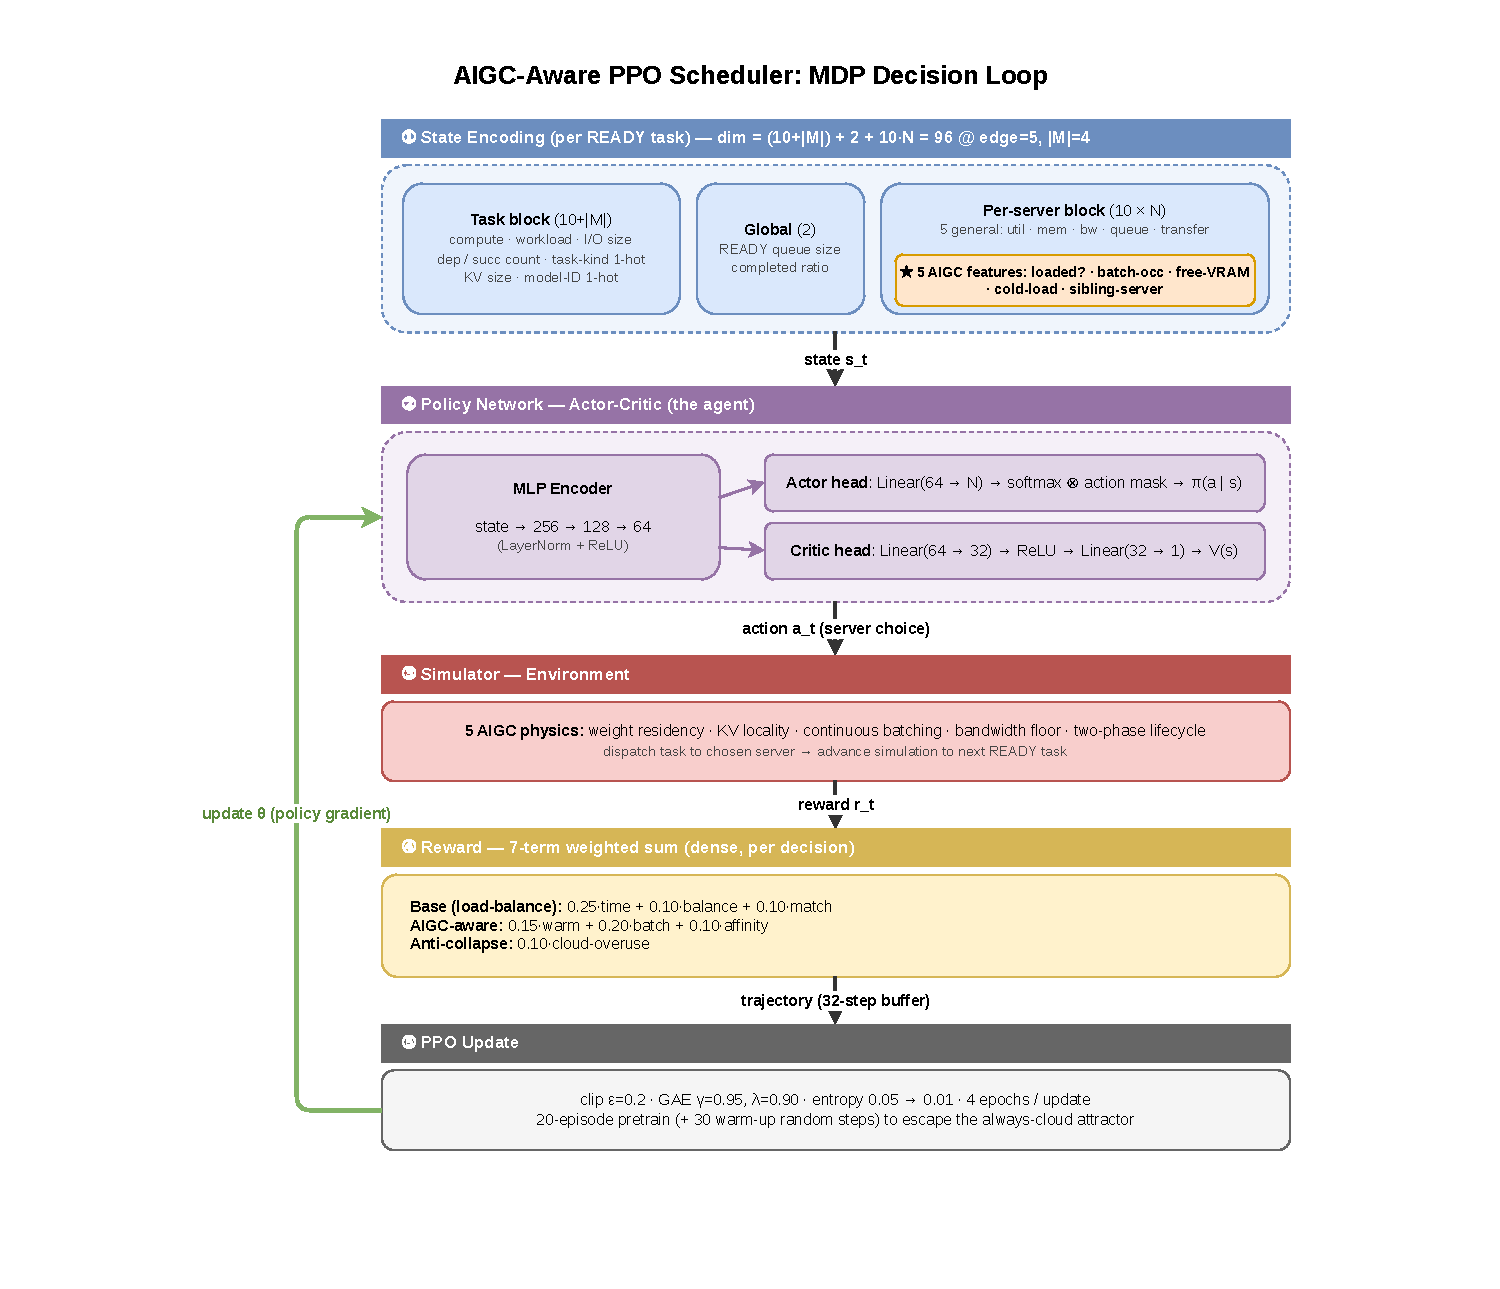
\includegraphics[width=0.66\textwidth]{rl_scheduler_arch.pdf}
  \caption{AIGC 感知 PPO 调度器的 MDP 决策闭环。对每个 \texttt{READY} 任务，状态编码器（\textcircled{1}）构建 96 维向量，其每服务器块携带五个 AIGC 特定特征（高亮）；actor-critic 策略（\textcircled{2}）输出带掩码的动作分布与价值估计；所选服务器被派发进仿真器（\textcircled{3}，五项 AIGC 物理）；7 项稠密奖励（\textcircled{4}）分为负载均衡、AIGC 感知与防坍缩三组；PPO 更新（\textcircled{5}）经策略梯度闭合回路。预训练正是让策略跳出 always-cloud 吸引子的关键。}
  \label{fig:rl-arch}
\end{figure*}

\textbf{状态。}对每个 \texttt{READY} 任务，编码器输出维度为 $(10+|\mathcal{M}|)+2+10N$ 的扁平向量：\emph{任务块}（计算需求、工作量、输入/输出大小、依赖计数、任务类型与模型 ID one-hot、归一化 KV 大小），2 维\emph{全局块}（队列长度、已完成比例），以及 $10$ 维的每服务器块，含五个通用特征（算力/显存利用率、带宽、队列长度、传输时间估计）与五个\textbf{AIGC 特定特征}：（i）已加载模型指示、（ii）归一化批占用率、（iii）剩余显存比例、（iv）归一化冷加载代价、（v）\emph{兄弟服务器指示}---对 Decode 任务，标记候选服务器是否就是 Prefill 运行的那台，使策略无需对请求 ID 进行推理即可直接读取 KV cache 本地性。当 edge${=}5$、$|\mathcal{M}|{=}4$ 时，状态维度为 96。

\textbf{动作。}在 $N$ 台服务器上离散选择，配以\textbf{动作掩码}（凡 \texttt{can\_allocate} 失败的服务器其概率清零）；掩码在每次分派时重算。

\textbf{奖励。}7 项稠密的逐决策奖励分量加权求和：
\begin{equation}
  \label{eq:reward}
  \begin{aligned}
    r =\;& 0.25\,r_{\text{time}}
        + 0.10\,r_{\text{balance}}
        + 0.10\,r_{\text{match}} \\
       &+ 0.15\,r_{\text{warm}}
        + 0.20\,r_{\text{batch}} \\
       &+ 0.10\,r_{\text{affinity}}
        + 0.10\,r_{\text{cloud}},
  \end{aligned}
\end{equation}
将三项负载均衡信号（$r_{\text{time}}$、$r_{\text{balance}}$、$r_{\text{match}}$ 分别惩罚长完成时间、服务器过载与算力不匹配）与四项 AIGC 特定信号相结合：$r_{\text{warm}}$（模型已加载时 $+1$，否则取 $-\text{cold\_load}/20$ 并 clip 至 $[-1,0]$）；$r_{\text{batch}}$ 鼓励加入同模型已有批（Decode 权重更高）；$r_{\text{affinity}}$ 在 Decode 与其 Prefill 同址时奖励 $+1$，在 KV 迁移成本非平凡时惩罚 $-0.5$；$r_{\text{cloud}}$（存在可行边缘替代时取 $-u_{\text{cloud}}$）抑制我们在早期实验中观察到的"always-cloud"吸引子（见 \S\ref{sec:implications}）。
典型权重将 0.45 分配给负载均衡组、0.45 分配给 AIGC 组、0.10 分配给防坍缩惩罚；组内各权重大致按各信号在诊断实验中的信息量比例设定。我们强调这一选择\emph{并非}精细调优：在从延迟优先到 AIGC 优先的四组备选权重向量下重新训练，两个目标在统计上均无变化（\S\ref{sec:weight-sens}）。

\textbf{网络结构与训练。}3 层多层感知机（MLP）编码器（$\text{state} \to 256 \to 128 \to 64$，LayerNorm + ReLU）接入 Actor 头（Linear $\to$ 带掩码 softmax）与 Critic 头（Linear $\to$ ReLU $\to$ Linear）。我们以 PPO~\cite{schulman2017ppo} 训练（clip $\epsilon{=}0.2$）、GAE~\cite{schulman2015gae}（$\gamma{=}0.95$、$\lambda{=}0.90$）与熵正则（系数 $0.05$，预训练后降至 $0.01$）；每次更新使用 32 条缓存 transition、4 个 epoch。关键地，我们在在线训练前进行 \textbf{20 个 episode 的预训练}（约 10--15~s 墙钟），起手 30 步使用均匀随机动作 warm-up 初始化；若无此预训练，策略会坍缩到"always-cloud"，\slo{} 下降 $38\%$（\S\ref{sec:ablation}）。每个 AIGC 组件由构造器开关控制，从而支持 \S\ref{sec:ablation} 的 12 组件消融。

% =============================================================
% §5 实验评估
% =============================================================
\section{实验评估}
\label{sec:eval}

\subsection{实验设置}
\label{sec:eval-setup}

\textbf{仿真平台。}所有实验均使用 \S\ref{sec:simulator} 的仿真器，其以里程碑 M1--M4 实现五项 AIGC 物理。

\textbf{硬件配置。}1 台云级服务器（200~TFLOPS，128~GB 显存，等效 A100-80GB）+ 1--7 台异构边缘节点（10--50~TFLOPS，16--64~GB 显存，对照 Jetson AGX、T4、边缘 A100 部署建模）。云--边链路网络延迟 30--65~ms，边--边链路 8--23~ms。

\textbf{工作负载。}采用与 Azure LLM Inference Trace 2023~\cite{azure2023llmtrace} 公开统计对齐的对数正态请求长度分布：prompt 长 $\sim \text{LogNormal}(\mu{=}5.5, \sigma{=}1.0)$，输出长 $\sim \text{LogNormal}(\mu{=}4.5, \sigma{=}1.2)$。请求到达为速率 $\lambda$ 的 Poisson 过程。每个请求在三种模型（LLaMA-7B、LLaMA-13B、LLaMA-70B-INT8）中均匀采样，模型参数标定至 vLLM 与 TensorRT-LLM 的基准数据。

\textbf{基线（11 种调度器）。}对比覆盖广泛：
\begin{itemize}
\item \textbf{RoundRobin（RR）}---无负载感知基线。
\item \textbf{LeastLoaded（LL）}---负载感知贪心。
\item \textbf{ShortestQueue（SQ）}---队列感知贪心。
\item \textbf{HEFT}~\cite{topcuoglu2002heft}---标准 DAG 调度基线。
\item \textbf{GA}~\cite{holland1975adaptation}、\textbf{PSO}~\cite{kennedy1995pso}---元启发式搜索。
\item \textbf{NSGA-II}~\cite{yu2025llmrouting}---多目标遗传搜索（非支配排序 + 拥挤距离），在逐窗口分配上进行，两个目标与本文两轴对应（完成时间代理、能耗估计）；执行最终 Pareto 前沿的 knee point 解。
\item \textbf{A3C-R2N2}~\cite{tuli2022a3cr2n}---RL 基线，采用异步优势 actor-critic 与 GRU+残差编码器，但使用\textbf{通用（非 AIGC）状态与奖励}。
\item \textbf{GNN}---本文调度器的 graph-neural-network 变体，将 AIGC 物理编码为任务--服务器二部图中的\textbf{边特征}，与 Decima~\cite{mao2019decima} 类似。
\item \textbf{CS-UCB}~\cite{yang2024perllm}---PerLLM 风格的约束满足 UCB bandit，最接近的先行工作（\S\ref{sec:related}）：在可行 arm 中按最大 UCB 逐请求选择服务器，奖励为 $-E_{\text{est}} + \lambda f(y)$（负能耗估计加归一化约束裕量）。
\item \textbf{RL（本文）}---本文的 AIGC 感知 PPO 调度器，含显式 AIGC 状态特征与奖励整形。
\end{itemize}

全部 11 种调度器均以 Python 原生实现，对接仿真器统一的 \texttt{scheduler.schedule()} 接口；未复用任何外部调度器库。NSGA-II 基线复现~\cite{yu2025llmrouting} 的多目标云边路由设定。HEFT 遵循原始的 upward-rank 公式~\cite{topcuoglu2002heft}；A3C-R2N2 复现~\cite{tuli2022a3cr2n} 的 GRU + 残差跳连网络；GNN 变体采用 Decima 风格的图编码~\cite{mao2019decima}；CS-UCB 在本文的逐任务粒度上复现 PerLLM 的约束满足 UCB~\cite{yang2024perllm}，以 (model, phase, server) 逐组维护的 arm 统计对应其按服务的个性化。表~\ref{tab:hyperparams} 列出各调度器的超参数与搜索/训练预算；所有实现随本文开源发布。

\begin{table}[t]
  \centering
  \caption{调度器实现与超参数。RR/LL/SQ = RoundRobin、LeastLoaded、ShortestQueue。}
  \label{tab:hyperparams}
  \small
  \setlength{\tabcolsep}{4pt}
  \begin{tabular}{@{}l@{\hspace{6pt}}p{0.64\columnwidth}@{}}
    \toprule
    Scheduler & Configuration \\
    \midrule
    RR / LL / SQ & 无参数贪心规则 \\
    HEFT & upward rank + earliest finish time；无参数 \\
    GA & 每调度窗口 population 30、50 代；交叉 0.8、变异 0.1、精英保留 0.1 \\
    PSO & 每窗口 30 粒子、30 次迭代；惯性 $w{=}0.7$、$c_1{=}c_2{=}1.5$ \\
    NSGA-II & 每窗口 population 30、30 代；交叉 0.8、变异 0.1；执行最终非支配前沿的 knee point 解 \\
    A3C-R2N2 & GRU 单元 + 残差跳连（隐层 128）；Adam $3{\times}10^{-4}$、$\gamma{=}0.95$、熵系数 0.05、value 系数 0.5；每 32 个 transition 更新一次（单 epoch、无裁剪，按~\cite{tuli2022a3cr2n}） \\
    GNN & 任务--服务器二部图上的 1-hop 注意力消息传递（隐层 64）；与本文相同的 PPO 配方与预算 \\
    CS-UCB & arm = (model, phase, server)；以准入检查作可行性过滤；探索系数 $\delta{=}0.5$、约束权重 $\lambda{=}1.0$（在 $\delta \in \{0.1,\dots,2\}$、$\lambda \in \{0.5,1\}$ 上网格调参） \\
    RL（本文） & MLP $256{\to}128{\to}64$；PPO 裁剪 $\epsilon{=}0.2$、GAE $\gamma{=}0.95$、$\lambda{=}0.90$；Adam $3{\times}10^{-4}$；熵系数在预训练后 $0.05{\to}0.01$；每 32 个 transition $\times$ 4 epoch 更新 \\
    \addlinespace
    \multicolumn{2}{@{}p{0.97\columnwidth}@{}}{\emph{训练预算（所有学习型调度器）：}20 个预训练 episode + 30 次随机 warm-up 派发；评估期间在线更新持续进行。} \\
    \bottomrule
  \end{tabular}
\end{table}

\textbf{指标。}沿用标准 LLM 服务基准：\slo{} 达成率（满足 TTFT $\le$ 2.0~s 且 TPOT $\le$ 100~ms/token 的比例）；TTFT 与 TPOT 百分位；goodput；总能耗；以及每 token 能耗（J/tok），采用 \S\ref{sec:simulator} 标定的功率模型。

\textbf{统计方法。}所有实验使用 30 个独立随机种子；报告均值~$\pm$~标准差，并以双侧 Mann-Whitney U 检验显著性（仿真输出非高斯）。阈值：$*$ $p<0.05$，$**$ $p<0.01$，$***$ $p<0.001$。

\subsection{主结果：Pareto 占优}
\label{sec:main-results}

我们在典型配置上评估全部 11 种调度器：5 台服务器（1 云 + 4 异构边缘）、Poisson 到达 $\lambda{=}2$ 请求/秒、100 个任务单位（约 50 个推理请求）。结果按 30 次运行取均值。

\textbf{核心结论。}本文 AIGC 感知 RL 调度器同时取得最高 \slo{} 达成率\textbf{与}最低每 token 能耗，在 (\slo, 能效) 平面上\textbf{按均值表现 Pareto 占优全部 10 个基线}（表~\ref{tab:main}，图~\ref{fig:pareto}）。

\begin{table}[t]
  \centering
  \caption{典型配置（edge${=}5$、$\lambda{=}2$ 请求/秒、$N{=}30$）下的主对比。Mksp.\ = makespan（s）；E = 总能耗（kJ）；\etok{} = 每 token 能耗（J）；TTFT P95 单位为秒。粗体 = 列最优。}
  \label{tab:main}
  \scriptsize
  \setlength{\tabcolsep}{3pt}
  \begin{tabular}{lrrrrr}
    \toprule
    Scheduler & Mksp.(s) & \slo$\uparrow$ & E(kJ)$\downarrow$
              & \etok(J)$\downarrow$ & TTFT P95 \\
    \midrule
    RoundRobin    & 306.2 & 0.163 & 64.0 & 7.29 & 174.6 \\
    LeastLoaded   & 125.5 & 0.239 & 26.8 & 2.94 & 30.8 \\
    ShortestQueue & 123.8 & 0.234 & 26.9 & 2.96 & 25.4 \\
    HEFT          & 126.7 & 0.169 & 25.9 & 2.83 & 35.7 \\
    GA            & 132.4 & 0.225 & 26.9 & 2.94 & 30.5 \\
    PSO           & 129.6 & 0.235 & 25.6 & 2.81 & 41.0 \\
    A3C-R2N2      & \textbf{120.6} & 0.214 & 26.7 & 2.93 & 28.8 \\
    GNN           & 125.5 & 0.210 & 26.7 & 2.93 & 32.2 \\
    CS-UCB        & 129.9 & 0.193 & 26.0 & 2.84 & 37.3 \\
    NSGA-II       & 126.2 & 0.289 & 25.5 & 2.79 & 32.0 \\
    \textbf{RL（本文）} & 122.2 & \textbf{0.302}
                       & \textbf{23.7} & \textbf{2.61}
                       & \textbf{25.2} \\
    \bottomrule
  \end{tabular}
\end{table}

本文 RL 调度器在除 makespan 外的每项指标上均为最优；makespan 一项由 A3C-R2N2 略早完成（120.6~s vs.\ 122.2~s，差距 1.3\%）。makespan 不在本文优化目标之列（\S\ref{sec:sched-problem}），该差距也不影响 (\slo, \etok) 平面上的 Pareto 关系。

\begin{figure}[t]
  \centering
  \includegraphics[width=\columnwidth]{fig4_pareto.pdf}
  \caption{典型配置（edge${=}5$、$\lambda{=}2$ 请求/秒、$N{=}30$）下 \slo{} 达成率 vs.\ 每 token 能耗的 Pareto 图。“理想”角位于左上。本文 RL 调度器单独占据该区域。单目标基线聚集在右下且 \slo{} 明显更低；最接近的挑战者 NSGA-II 在两个轴上均落后。RoundRobin 是图外的极端离群点。}
  \label{fig:pareto}
\end{figure}

\textbf{显著性检验。}表~\ref{tab:significance} 报告本文 RL 调度器对 6 个最强基线的 Mann-Whitney U 检验。

\begin{table}[t]
  \centering
  \caption{对 6 个最强基线的 $p$ 值（双侧 Mann-Whitney U，$N{=}30$）。粗体 = $p<0.05$。}
  \label{tab:significance}
  \scriptsize
  \setlength{\tabcolsep}{2.5pt}
  \begin{tabular}{lcccccc}
    \toprule
    Metric & PSO & SQ & A3C-R2N2 & GNN & CS-UCB & NSGA-II \\
    \midrule
    \slo{} 达成      & \textbf{0.045}$^*$ & \textbf{0.046}$^*$
                     & \textbf{0.006}$^{**}$ & \textbf{0.006}$^{**}$
                     & \textbf{0.002}$^{**}$ & 0.64 \\
    总能耗           & 0.36 & 0.07 & 0.09 & 0.10 & 0.21 & 0.27 \\
    每 token 能耗    & 0.11 & \textbf{0.010}$^{**}$
                     & \textbf{0.028}$^*$ & \textbf{0.016}$^*$
                     & 0.066 & 0.12 \\
    \bottomrule
  \end{tabular}
\end{table}

\slo{} 达成率维度上，本文调度器对全部 5 个单目标基线均显著更高（$p<0.05$，其中对两个 DRL 基线与 bandit 均为 $p<0.01$）。能效维度对 6 个中的 3 个显著更优（PSO，$p=0.11$，与 CS-UCB，$p=0.066$，方向一致但未达 $p<0.05$）。在该工作点上唯一未能与本文调度器统计分离的基线是 NSGA-II（\slo{} $p=0.64$、\etok{} $p=0.12$）：本文在两个均值上均更好，但在 $N{=}30$ 下差距处于噪声之内；下文将回到这一对比---包括其甜区显著性与代价不对称性。总能耗维度展示出一致的 $\le 10\%$ 优势但未达单独显著，反映了 makespan 与能耗之间预期的相关性。

\textbf{为何 AIGC 感知 RL 能耗更低？}反直觉的是，本文调度器---尽管可以调用高功率云端资源---比默认偏向边缘的基线消耗\emph{更少}的能量。我们将其归因于三种学到的行为：（i）\emph{更短 makespan 放大空闲节能}（集群空闲功率约 150~W）；（ii）\emph{冷加载规避}---将同模型请求集中放置，消除了让 GPU 通电却不产 token 的加载时段；（iii）\emph{兄弟亲和}---decode 与其 prefill 同址放置，避免了“通电空转”的 KV 传输区间。\textbf{当能耗作为协同目标时，这些行为使 AIGC 感知设计呈现 Pareto 占优。}

\textbf{与 A3C-R2N2 对照（RL 主干受控对比）。}A3C-R2N2 使用相同的 actor-critic 框架，但（a）编码器为 GRU+残差而非本文的 MLP，（b）状态与奖励为通用设计、不含 AIGC 成分。这是受控程度最高的对比。A3C-R2N2 取得 \slo${} = 0.214 \pm 0.07$、\etok${} = 2.93$~J/tok，本文为 $0.302 \pm 0.07$ 与 $2.61$~J/tok。差异在 \slo{} 维度 $p<0.01$、\etok{} 维度 $p<0.05$ 下显著。由于主干等价（均为带充足预训练的 actor-critic），这 $41\%$ 的 \slo{} 提升与 $11\%$ 的能效提升\textbf{可直接归因于 AIGC 感知的状态与奖励设计}。

\textbf{与 GNN 对照（状态编码受控对比）。}GNN 变体将 AIGC 物理编码为任务--服务器二部图中的\textbf{边特征}，是本文“MLP + 扁平 AIGC 特征”的替代方案。尽管架构更复杂，GNN 仅取得 \slo${} = 0.210 \pm 0.08$、\etok${} = 2.93$~J/tok，与 A3C-R2N2 基本持平，显著弱于本文调度器（$p<0.01$ \slo、$p<0.05$ \etok）。我们将该差距归因于\textbf{训练数据效率}：GNN 的关系推理能力需要比预训练预算（20 episode）更多的样本才能充分专门化。

\textbf{与 CS-UCB 对照（PerLLM 风格 bandit）。}CS-UCB 与本文共享逐请求粒度与能耗目标，其约束满足机制对应 PerLLM~\cite{yang2024perllm}。但它落在基线簇中（\slo{} 0.193、\etok{} 2.84）：\slo{} 显著低于本文调度器（$p{=}0.002$），能耗方向性更差（$p{=}0.066$）。原因是结构性的：平稳的逐 arm 均值无法跟踪\emph{状态相关}的代价---模型驻留与批处理槽位取决于集群不断演化的状态，上下文无关的 bandit 将其平均掉，而深度策略以其为条件。约束过滤不能替代基于状态的学习。

\textbf{与 NSGA-II 对照（多目标搜索）。}NSGA-II 是目前为止最强的基线，值得坦率分析。它在逐窗口分配上针对与本文相同的两个目标进行搜索，在典型工作点取得 \slo{} 0.289、\etok{} 2.79---本文调度器在两个均值上均更好（0.302、2.61），但在 $N{=}30$ 下两个差距均未单独显著（$p=0.64$、$p=0.12$）。三点观察补全图景。第一，在\textbf{中等负载甜区}中分离是真实的：$\lambda{=}1$ 处本文 \slo{} 达 0.447，NSGA-II 为 0.352（相对 $+27\%$，$p=0.009$）。第二，在我们运行 NSGA-II 的\textbf{全部八个配置中，本文每 token 能耗均更低}，优势从 $\lambda{=}0.5$ 处的持平增长到高负载下的 7--9\%。第三，两者在\textbf{调度时代价}上不对称：NSGA-II 在派发时刻重新运行种群搜索（总 wall-clock 为本文的 $5.4\times$；实测每派发一个任务约 70~ms 搜索），而本文策略经一次性预训练后以亚毫秒前向推理决策---在延迟敏感的服务场景中，派发时搜索恰恰会推高它所要保护的 TTFT。因此我们将 NSGA-II 视为最强的\emph{离线}竞争者；其在饱和工况的强势（\S\ref{sec:load}）使工况刻画（C4）更加清晰。

\subsection{拓扑敏感性}
\label{sec:topology}

在固定 $\lambda{=}2$ 请求/秒与 uniform 模型混合下，将边缘服务器数从 3 变到 7（始终配 1 台云端）。表~\ref{tab:topology} 报告 4 个最强基线与本文调度器的 \slo{} 与 \etok{}。

\begin{table}[t]
  \centering
  \caption{\slo{} 与 \etok{}（J/tok）随边缘数量变化。$\bigstar$ = 全部 11 种调度器中的列最优。}
  \label{tab:topology}
  \scriptsize
  \setlength{\tabcolsep}{2pt}
  \begin{tabular}{lrrrrrrr}
    \toprule
    配置（1 云 +）
      & PSO & SQ & A3C-R2N2 & GNN & CS-UCB & NSGA-II & \textbf{RL} \\
    \midrule
    3 边 --- \slo
      & 0.273 & 0.277 & 0.246 & 0.241 & 0.243 & 0.296
      & \textbf{0.314}$^\bigstar$ \\
    3 边 --- \etok
      & 2.19 & 2.32 & 2.28 & 2.24 & 2.24 & 2.16
      & \textbf{1.99}$^\bigstar$ \\
    5 边 --- \slo
      & 0.235 & 0.234 & 0.214 & 0.210 & 0.193 & 0.289
      & \textbf{0.302}$^\bigstar$ \\
    5 边 --- \etok
      & 2.81 & 2.96 & 2.93 & 2.93 & 2.84 & 2.79
      & \textbf{2.61}$^\bigstar$ \\
    7 边 --- \slo
      & 0.241 & 0.218 & 0.193 & 0.250 & 0.152 & 0.277
      & \textbf{0.282}$^\bigstar$ \\
    7 边 --- \etok
      & 3.25 & 3.34 & 3.35 & 3.35 & 3.35 & 3.19
      & \textbf{3.00}$^\bigstar$ \\
    \bottomrule
  \end{tabular}
\end{table}

在全部三种拓扑配置下，本文 RL 调度器在每项指标上均为最优。相对单目标基线，RL 的 \slo{} 相对领先 13--28\%、能耗领先 7--9\%。最强挑战者 NSGA-II 将 \slo{} 差距收窄到相对 2--6\%，但在每种拓扑下每 token 能耗都要多付 6--8\%---与我们在典型工作点观察到的不对称相同。

\textbf{能效优势比 \slo{} 更“配置稳定”。}相对能效提升在全部拓扑配置下都落在 [7\%, 9\%] 的窄带内，而 \slo{} 提升波动更大（13--28\%）。这表明\textbf{能效比 \slo{} 更干净地刻画了 AIGC 感知调度的“内在”收益}：\slo{} 对集群争用动态敏感，而能耗直接反映每任务效率。

\subsection{负载敏感性}
\label{sec:load}

固定 edge${=}5$，扫描 Poisson 到达率 $\lambda \in \{0.5, 1, 2, 4, 8\}$ 请求/秒，刻画调度器行为从欠利用到过饱和的变化。表~\ref{tab:slo-vs-lambda} 报告整个扫描范围内的 \slo{} 达成率与每 token 能耗。

\begin{table}[t]
  \centering
  \caption{负载扫描：\slo{} 达成率（上）与每 token 能耗（J/tok，下）随到达率变化。$\bigstar$ = 严格胜出；$\dagger$ = 与 PSO 持平。}
  \label{tab:slo-vs-lambda}
  \scriptsize
  \setlength{\tabcolsep}{2pt}
  \begin{tabular}{rrrrrrrl}
    \toprule
    $\lambda$ & PSO & SQ & A3C-R2N2 & GNN & CS-UCB & NSGA-II
      & \textbf{RL} \\
    \midrule
    \multicolumn{8}{@{}l}{\emph{\slo{} 达成率}} \\
    0.5 & 0.596 & 0.339 & 0.359 & 0.500 & 0.462 & 0.577
        & \textbf{0.596}$^\dagger$ \\
    1.0 & 0.297 & 0.265 & 0.227 & 0.237 & 0.214 & 0.352
        & \textbf{0.447}$^\bigstar$ \\
    2.0 & 0.235 & 0.234 & 0.214 & 0.210 & 0.193 & 0.289
        & \textbf{0.302}$^\bigstar$ \\
    4.0 & 0.253 & 0.205 & 0.191 & 0.207 & 0.215
        & \textbf{0.267} & 0.214 \\
    8.0 & 0.216 & 0.167 & 0.156 & 0.193 & 0.187
        & \textbf{0.219} & 0.199 \\
    \addlinespace
    \multicolumn{8}{@{}l}{\emph{每 token 能耗（J/tok）}} \\
    0.5 & 3.00 & 3.49 & 3.38 & 3.13 & 3.19 & 2.97
        & \textbf{2.96}$^\bigstar$ \\
    1.0 & 2.77 & 3.00 & 3.07 & 2.95 & 2.93 & 2.84
        & \textbf{2.64}$^\bigstar$ \\
    2.0 & 2.81 & 2.96 & 2.93 & 2.93 & 2.84 & 2.79
        & \textbf{2.61}$^\bigstar$ \\
    4.0 & 2.85 & 2.97 & 2.94 & 2.92 & 2.86 & 2.78
        & \textbf{2.58}$^\bigstar$ \\
    8.0 & 2.94 & 2.89 & 2.98 & 2.91 & 2.99 & 2.78
        & \textbf{2.52}$^\bigstar$ \\
    \bottomrule
  \end{tabular}
\end{table}

\textbf{关键观察。}（1）\emph{能效维度在所有负载下均为 RL 占优。}RL 在每个 $\lambda$ 都取得最低每 token 能耗（5/5），且相对次优基线的优势随负载单调增长---从 $\lambda{=}0.5$ 处的持平到 $\lambda{=}8$ 处的 $9\%$。（2）\emph{\slo{} 占优集中于中等负载工况}（$\lambda \in [0.5, 2]$）：在每一点 RL 均严格胜出或持平；$\lambda{=}1$ 处相对最强基线（NSGA-II，$p=0.009$）提升 $27\%$、相对 PSO 提升 $50\%$。（3）\emph{在极高负载下（$\lambda \ge 4$）}，集群逼近其物理吞吐上限，离线多目标搜索接管 \slo{} 轴：NSGA-II 在 $\lambda{=}4$ 与 $\lambda{=}8$ 处严格胜出，PSO 紧随其后---批量搜索比任何增量式策略更能利用同质化的队列状态---甚至 CS-UCB 也在 $\lambda{=}4$ 处达到 RL 的 \slo{} 水平（0.215 vs.\ 0.214）。\textbf{但 RL 的能效优势在该工况下持续存在且达到峰值}（表~\ref{tab:slo-vs-lambda} 下块）。

\textbf{AIGC 感知设计在什么工况下最有用？}我们刻画三个工况：\textbf{轻载}（$\lambda \le 1$，资源有余）---两轴均最优或持平；\textbf{甜区}（$1 \le \lambda \le 2$）---严格 Pareto 胜出，且 $\lambda{=}1$ 处的 \slo{} 领先即使相对 NSGA-II 也显著；\textbf{饱和}（$\lambda \ge 4$，吞吐上限）---仅保有能效优势，\slo{} 轴让位于离线多目标搜索。这一细致结论比扁平的“我们到处赢”更可辩护。最干净的表述是：\emph{AIGC 感知 RL 在每个负载下都取得最低每 token 能耗---且优势随负载增长---并在刻画多数生产推理部署的中等负载工况下取得严格的 \slo{}+能耗 Pareto 占优}。

\subsection{工作负载组合敏感性}
\label{sec:workload}

在 edge${=}5$、$\lambda{=}2$ 下测试两种模型混合：\textbf{uniform}（LLaMA-7B/13B/70B 各 1/3）与 \textbf{large-heavy}（70\% LLaMA-70B-INT8，偏向显存受限请求）。表~\ref{tab:workload} 报告结果。

\begin{table}[t]
  \centering
  \caption{不同工作负载混合下的 Pareto 表现。}
  \label{tab:workload}
  \small
  \begin{tabular}{llrr}
    \toprule
    Mix & Scheduler & \slo{} & \etok{} \\
    \midrule
    uniform & PSO            & 0.235 & 2.81 \\
    uniform & ShortestQueue  & 0.234 & 2.96 \\
    uniform & A3C-R2N2       & 0.214 & 2.93 \\
    uniform & GNN            & 0.210 & 2.93 \\
    uniform & CS-UCB         & 0.193 & 2.84 \\
    uniform & NSGA-II        & 0.289 & 2.79 \\
    uniform & \textbf{RL（本文）}
            & \textbf{0.302}$^\bigstar$ & \textbf{2.61}$^\bigstar$ \\
    \midrule
    large-heavy & PSO            & 0.093 & 3.84 \\
    large-heavy & ShortestQueue  & 0.105 & 3.84 \\
    large-heavy & A3C-R2N2       & 0.107 & 3.79 \\
    large-heavy & GNN            & 0.091 & 3.79 \\
    large-heavy & CS-UCB         & 0.068 & 3.84 \\
    large-heavy & NSGA-II        & \textbf{0.122} & 3.68 \\
    large-heavy & \textbf{RL（本文）}
                & 0.098 & \textbf{3.58}$^\bigstar$ \\
    \bottomrule
  \end{tabular}
\end{table}

在 \textbf{uniform 混合}下，本文 RL 为严格 Pareto 胜出者。在 \textbf{large-heavy 混合}下图景改变：所有调度器的 \slo{} 都坍缩到一个低带（0.07--0.12，uniform 下为 0.19--0.30），因为 LLaMA-70B-INT8（70~GB 权重）物理上\emph{只能装入云端服务器}。无论选择哪种调度器，云端队列都会饱和；在该带内，NSGA-II 的离线搜索取得最佳 \slo{}（0.122），呼应其在 \S\ref{sec:load} 中的饱和优势。\textbf{能效是唯一可广泛区分的轴}，RL 在该轴上仍然领先（3.58，对 NSGA-II 的 3.68 与其余基线的 3.79--3.84）。\emph{当工作负载在特定层级超出集群容量时，AIGC 感知调度退化为纯能效优化}（\S\ref{sec:discuss} 讨论）。

\subsection{组件消融}
\label{sec:ablation}

为隔离本文 RL 调度器的哪些组件贡献于其 Pareto 占优，我们系统消融 12 个组件：一次关闭一个、其余保持不变。所有消融使用 edge${=}5$、$\lambda{=}2$ 请求/秒、uniform 混合、$N{=}30$ 次运行。表~\ref{tab:ablation} 报告全部 12 个配置。

\textbf{消融分类。}四大类：\emph{物理层}（\texttt{no\_batching}）；\emph{PPO 内部}（\texttt{no\_action\_mask}、\texttt{no\_gae}、\texttt{no\_pretrain}、\texttt{no\_entropy}）；\emph{AIGC 奖励}（\texttt{no\_warm\_reward}、\texttt{no\_batch\_reward}、\texttt{no\_affinity\_reward}、\texttt{no\_cloud\_overuse}、\texttt{no\_all\_aigc\_rewards}）；\emph{AIGC 状态}（\texttt{no\_aigc\_state}、\texttt{no\_aigc\_full}）。

\begin{table*}[t]
  \centering
  \caption{组件消融。$\Delta$ 相对完整 RL（$N{=}30$、edge${=}5$、$\lambda{=}2$、uniform 混合）。$p$ 值来自对 \slo{} 相对完整 RL 的 Mann-Whitney U 检验。粗体 = $p<0.05$。}
  \label{tab:ablation}
  \small
  \begin{tabular}{llrrrrr}
    \toprule
    Category & Configuration & \slo{} & $\Delta$\slo\%
             & \etok{} & $\Delta$\etok\% & $p$(\slo) \\
    \midrule
    --- & \textbf{完整 RL（本文）}
        & \textbf{0.302} & ---
        & \textbf{2.61} & --- & --- \\
    \midrule
    \textbf{物理}
      & \textbf{$-$ 连续批处理}
      & \textbf{0.051} & \textbf{$-$83.2\%}
      & \textbf{5.75} & \textbf{$+$120.5\%}
      & \textbf{$<$0.001}$^{***}$ \\
    \textbf{PPO}
      & \textbf{$-$ 预训练（20$\to$0 ep）}
      & \textbf{0.186} & \textbf{$-$38.4\%}
      & \textbf{2.96} & \textbf{$+$13.5\%}
      & \textbf{$<$0.001}$^{***}$ \\
    PPO & $-$ 动作掩码
      & 0.274 & $-$9.3\% & 2.66 & $+$2.1\% & 0.39 \\
    PPO & $-$ GAE（改用 Monte-Carlo return）
      & 0.292 & $-$3.3\% & 2.61 & $-$0.1\% & 0.65 \\
    PPO & $-$ 熵正则
      & 0.305 & $+$0.9\% & 2.54 & $-$2.8\% & 0.92 \\
    AIGC 奖励 & $-$ Warm bonus
      & 0.300 & $-$0.7\% & 2.60 & $-$0.4\% & 0.87 \\
    AIGC 奖励 & $-$ Batch bonus
      & 0.311 & $+$3.1\% & 2.59 & $-$0.8\% & 0.87 \\
    AIGC 奖励 & $-$ Affinity bonus
      & 0.287 & $-$4.9\% & 2.64 & $+$1.3\% & 0.57 \\
    AIGC 奖励 & $-$ Cloud-overuse 惩罚
      & 0.309 & $+$2.2\% & 2.60 & $-$0.5\% & 0.96 \\
    AIGC 奖励（联合） & $-$ 所有 AIGC 奖励
      & 0.302 & $+$0.0\% & 2.62 & $+$0.5\% & 0.95 \\
    AIGC 状态 & $-$ AIGC 状态特征
      & 0.295 & $-$2.2\% & 2.55 & $-$2.1\% & 0.81 \\
    AIGC（联合） & $-$ 所有 AIGC 设计
      & 0.306 & $+$1.3\% & 2.52 & $-$3.3\% & 0.99 \\
    \bottomrule
  \end{tabular}
\end{table*}

\textbf{发现：两个主导组件与一个惊人的零结果。}

\textbf{发现 1：连续批处理是物理基础}（$p<0.001$、$\Delta$\slo${} = -83.2\%$、$\Delta$\etok${} = +120.5\%$）。关闭批处理使 \slo{} 坍缩到 5\%、每 token 能耗翻倍不止，印证了 Orca~\cite{yu2022orca} 与 Sarathi-Serve~\cite{agrawal2024sarathi} 将迭代级批处理视为基础性基础设施的强调。

\textbf{发现 2：充足预训练不可或缺}（$p<0.001$、$\Delta$\slo${} = -38.4\%$、$\Delta$\etok${} = +13.5\%$）。没有预训练，放置策略坍缩向云端服务器---与既有观察（Decima~\cite{mao2019decima}、RLScheduler~\cite{zhang2020rlscheduler}）一致：在随机调度环境中 warm-start 不可或缺。

\textbf{发现 3：单一 AIGC 组件无显著效应}（所有 $p > 0.39$）。关闭任何单个 AIGC 组件产生的变化都在噪声范围内（$\pm 5\%$）---与如下解释一致：在充足基础特征与预训练下，PPO 会\emph{隐式学到} AIGC 感知行为，显式整形提供的是冗余信号。

\textbf{发现 4（最惊人）：去掉\emph{全部} AIGC 设计同样没有影响}（\slo{} 的 $p=0.99$，$\Delta$\etok${} = -3.3\%$）。联合消融 \texttt{no\_aigc\_full} 的 \slo{} 表现与完整 RL 基本相同，能效甚至\emph{略好}。结合 \S\ref{sec:main-results} 中“本文调度器 Pareto 占优十个基线---但其 AIGC 专属设计组件却可被单独乃至联合消融”的发现，这描绘出一幅更微妙的图景：\textbf{“AIGC 感知”的贡献体现在训练流程 + 仿真器物理 + RL 主干选择之中，而非任何单一奖励或状态组件}（图~\ref{fig:ablation}）。

\begin{figure*}[t]
  \centering
  \includegraphics[width=0.88\textwidth]{fig7_ablation.pdf}
  \caption{12 个配置的组件消融。左：$\Delta$\slo\% vs.\ 完整 RL；右：$\Delta$\etok\%。红条 = $p<0.05$；灰条 = 噪声范围内；浅灰带 = $\pm 10\%$。只有连续批处理与预训练显示统计显著效应；所有单一 AIGC 奖励与状态组件均在噪声范围内。}
  \label{fig:ablation}
\end{figure*}

\textbf{调和：为何 RL 能 Pareto 占优基线却对消融不敏感？}\S\ref{sec:main-results}（RL 在均值上占优 10 个基线）与表~\ref{tab:ablation}（无单一 AIGC 组件显著）之间的表面矛盾可这样化解：每个基线与本文调度器同时在\emph{多个}根本维度上不同（无学习；固定代价函数且不含 AIGC 物理；不同的编码器或训练配方）---因而落后 7--28\%。而当我们在本文调度器内部消融任何\emph{单个} AIGC 组件时，PPO 会从剩余特征中提取等价信号加以补偿。这告诉我们：\textbf{AIGC 感知调度是一项整体性的系统贡献，而非某个巧妙的奖励或状态组件}。

\subsection{奖励权重敏感性}
\label{sec:weight-sens}

式~\ref{eq:reward} 的奖励把一个多目标问题坍缩为标量加权和---我们的结论是否只是某个特定权重向量的产物？我们在覆盖设计空间的四种替代配置下从零重训---\emph{uniform}（全部权重 $1/7$）、\emph{time-heavy}（时间项占一半以上权重）、\emph{AIGC-heavy}（warm{+}batch{+}affinity 提升到 0.70）与 \emph{base-heavy}（AIGC 项几乎移除）---每种配置在典型工作点运行 $N{=}30$ 次（表~\ref{tab:weight-sens}）。

\begin{table}[t]
  \centering
  \caption{奖励权重敏感性（edge${=}5$、$\lambda{=}2$~请求/秒、每配置 $N{=}30$）。权重按式~\ref{eq:reward} 的 time/balance/match/warm/batch/affinity/cloud 顺序列出。$p$：对典型配置的双侧 Mann-Whitney U，\slo{} / \etok。每个配置均 Pareto 占优最强基线（PSO：\slo{}~0.235、\etok{}~2.81）。}
  \label{tab:weight-sens}
  \scriptsize
  \setlength{\tabcolsep}{2.5pt}
  \begin{tabular}{@{}llccc@{}}
    \toprule
    Config & Weights & \slo{} & \etok{} & $p$ \\
    \midrule
    canonical & .25/.10/.10/.15/.20/.10/.10
      & $0.302 {\pm} 0.13$ & $2.61 {\pm} 0.67$ & --- \\
    uniform & 各 $1/7$
      & $0.287 {\pm} 0.13$ & $2.61 {\pm} 0.68$ & .72 / .98 \\
    time-heavy & .55/.05/.05/.10/.10/.05/.10
      & $0.304 {\pm} 0.14$ & $2.60 {\pm} 0.67$ & .97 / .98 \\
    AIGC-heavy & .10/.05/.05/.25/.30/.15/.10
      & $0.300 {\pm} 0.12$ & $2.63 {\pm} 0.67$ & .86 / .96 \\
    base-heavy & .40/.20/.20/.05/.05/.05/.05
      & $0.305 {\pm} 0.14$ & $2.56 {\pm} 0.68$ & .89 / .74 \\
    \bottomrule
  \end{tabular}
\end{table}

两点观察。第一，\textbf{核心结论对权重选择稳健}：每个配置---包括极端配置---都 Pareto 占优最强基线（\slo{} 0.287--0.305 vs.\ PSO 的 0.235；\etok{} 2.56--2.63 vs.\ 2.81）。第二，\textbf{没有任何配置与典型权重存在显著差异}（所有 $p \ge 0.72$）：即便把 AIGC 组的权重质量从 0.15（base-heavy）移到 0.70（AIGC-heavy），两个目标在统计上均保持不变。这把消融的零结果从\emph{移除}组件扩展到\emph{重加权}组件，并说明我们的标量化是良性的：在权重空间的一个宽阔区域内，学到的策略落在同一个 Pareto 点上，因此从典型配置得出的结论具有普适性。

% =============================================================
% §6 讨论
% =============================================================
\section{讨论}
\label{sec:discuss}

\subsection{对 AIGC 调度研究的启示}
\label{sec:implications}

我们的实验支持三条超越 \S\ref{sec:eval} 所比较的具体调度器的启示。

\textbf{仿真器物理的影响力远超算法精巧度。}本研究中最大的效应---关闭连续批处理造成的 $-83\%$ \slo{} 坍缩（表~\ref{tab:ablation}）---比我们测得的任何奖励设计或状态工程选择都大一个数量级。研究精力与其投入网络架构或奖励公式，不如投入忠实的物理仿真。

\textbf{预训练是性价比最高的必备投资。}关闭预训练造成 $38\%$ \slo{} 跌幅（$p<0.001$），但只需 $20$ 个 episode（约 10--15~s 墙钟）即可。预训练的意义不在样本效率，而在于\textbf{跳出局部最优区域}：早期配置都陷入"always-cloud"吸引子，直到我们将充足预训练与 cloud-overuse 惩罚联合引入。

\textbf{勿过度归因于奖励整形。}一旦连续批处理与预训练就位，没有任何单一 AIGC 奖励项（乃至全部联合）能显著改善 \slo{}；权重敏感性研究（\S\ref{sec:weight-sens}）进一步表明，全部 7 项的\emph{相对权重}可从延迟优先切换到 AIGC 优先而无可测量的影响。先前声称某具体奖励项贡献的工作，可能忽略了充足表达力的 PPO 主干内部这种\textbf{可替换性}：缺少表~\ref{tab:ablation} 这类联合消融时，单项奖励的正向结果\emph{值得怀疑}。

总体上，这些启示提示 AIGC 调度研究议程应当从"造更好的奖励"转向\textbf{"造更好的仿真器与训练流程"}。

\subsection{局限与有效性威胁}
\label{sec:limitations}

\textbf{为何用仿真，及其保真度。}我们刻意选择在仿真中评估。本文的核心论断是\emph{比较性、统计性}的---一个必须在 30 种配置、每种 $N{=}30$ 个种子（共 900 次运行）上都成立的 Pareto 占优关系。在真实硬件上复现这一扫描，需要同时获得 A100、T4、Jetson 级节点并施加可控可复现的到达过程---而这恰是仿真器所隔离的场景：全部 11 种调度器跑在完全相同的负载与种子上，不受多租户、热降频、驱动漂移等混杂因素干扰。我们将仿真器常数（冷加载时间、批处理开销、显存带宽下限）标定至 vLLM 与 TensorRT-LLM 的公开实测值，使绝对量级而非仅相对量级保持真实。

尽管如此，仿真器有两处简化：将连续批处理建模为\emph{准入式}批处理而非 vLLM 的迭代级动态再批处理（在某些工况下可能低估真实批处理收益 10--20\%），并将显存带宽下限视为常数而非随 batch size 变化。因此我们把绝对消融量级（如 \texttt{no\_batching} 的 $-83\%$）理解为仿真器行为而非 vLLM 精确预测；而承载本文论断的效应\emph{排序}与\emph{显著性}对这些常数稳健。\textbf{在配备生产级推理引擎的物理云--边测试床上验证该 Pareto 关系，是最重要的未来工作}；我们开源的仿真器正是为让这一对比直接可行而设计：其 \texttt{scheduler.schedule()} 接口与真实派发器需实现的接口完全一致。

\textbf{工作负载与硬件覆盖。}我们的负载基于对齐 Azure 2023 的对数正态长度合成数据---未回放生产 trace，也未覆盖突发到达---硬件涵盖 A100/T4/Jetson 层级，但未含 H100 或定制加速器。所建模的定性物理特性架构无关；常数需对新硬件重新标定。

\textbf{统计功效与算法范围。}$N=30$ 次运行可检测中到大效应（Cohen's $d \ge 0.5$）；消融的零结果意味着"未能检测到大于 5\% 的 \slo{} 差异"，而非"不存在差异"。PPO、A3C-R2N2 与 GNN 变体均呈现类似的 AIGC 可替换性，但 offline RL / 基于模型的 RL 或模仿学习可能呈现不同响应。

\subsection{部署实践指导}
\label{sec:guidance}

本文结果提供四点实践指导。其一，\textbf{容量规划比调度器选择更重要}：当 70B 请求溢出唯一云端服务器时（\S\ref{sec:workload}），所有调度器 \slo{} 都被压到 ${\approx}10\%$---\emph{先备算力，再优调度}。其二，\textbf{中等负载工况下简单负载均衡器足矣}：LeastLoaded 与 ShortestQueue 以零训练成本达到 RL \slo{} 的 $78\%$。其三，\textbf{当能效、尾延迟或分派时间预算重要时再上 RL}：RL 在全部 30 种配置下取得最低 \etok{}（负载下优势最高达 9\%），其尾 TTFT（P95 25.2~s vs.\ 28--41~s）适合交互式服务，且其亚毫秒级策略推理避免了 NSGA-II 类调度器在请求路径上每次分派 $\approx$70~ms 的搜索开销。其四，\textbf{对奖励工程的声明保持怀疑}：若无针对含预训练基线的联合消融，增益可能反映通用 RL 主干的提升，而非所声称的机制。

% =============================================================
% §7 相关工作
% =============================================================
\section{相关工作}
\label{sec:related}

\textbf{LLM 服务系统（单机或集群内）。}Orca~\cite{yu2022orca} 引入迭代级连续批处理；vLLM~\cite{kwon2023vllm} 加入 PagedAttention 以实现非连续 KV 分配（吞吐 $2$--$4\times$）；Sarathi-Serve~\cite{agrawal2024sarathi} 引入分块 prefill 以缓解混合批中的生成阻塞。VoltanaLLM~\cite{yu2025voltana} 在 prefill/decode 解耦的集群内部，通过频率控制与状态空间路由协同优化能耗与 \slo{}。这些系统优化的是单个服务引擎或集群\emph{内部}的行为，与本文的跨服务器调度\textbf{正交}：本文的准入式批处理是它们迭代级批处理的一个可计算抽象，本文的逐请求放置决策可无改地传入 vLLM 风格引擎。

\textbf{集群调度：从启发式到学习。}经典调度器——按上行 rank 排定优先级的 HEFT~\cite{topcuoglu2002heft}，以及 GA~\cite{holland1975adaptation}、PSO~\cite{kennedy1995pso} 等元启发式——针对通用 DAG 负载优化固定代价模型；产业界则偏好更简单的负载均衡原语。学习式调度器随之出现：Decima~\cite{mao2019decima}（Spark DAG 上的 GNN + REINFORCE）、RLScheduler~\cite{zhang2020rlscheduler}（HPC 批作业），以及 A3C-R2N2~\cite{tuli2022a3cr2n}（面向通用边缘--云任务的 actor-critic，早于 LLM 时代）——后者是部署拓扑上最接近的前驱，我们将其作为\textbf{对照基线}进行基准比较（\S\ref{sec:main-results}）以隔离本文的 AIGC 贡献。这一路线至今活跃：近期工作将基于 GNN 的 DRL 用于能耗感知云调度~\cite{dagtopology2026}，将扩散辅助的奖励塑形用于跨数据中心的 AIGC 负载调度~\cite{aigcenergy2026}。该文献中的两个发现预示了本文结论：Decima 的收益集中在高集群负载下，而 \cite{dagtopology2026} 观察到每个学得策略都会退化为某一 regime 特定的启发式——与本文的 regime 刻画（C4）一致。这些调度器无一编码 LLM 服务物理。

\textbf{跨服务器的 LLM 请求调度。}一条快速增长的路线在实例\emph{之间}而非单引擎之内调度 LLM 推理。在单集群内部，Microsoft 的负载感知路由器~\cite{jain2024router} 在 prefill/decode 与批混合效应上训练启发式引导的 RL 策略；Lodestar~\cite{lim2026lodestar} 学习一个将批处理与 KV cache 复用耦合的在线奖励预测器——两者都呼应了本文"应把服务物理暴露给学习式路由器"的论点，但均未建模云--边层级或能耗。FREESH~\cite{he2025freesh} 通过经典优化在地理分布的异构 GPU 上为能耗与碳排放做路由与调度；MARLIN~\cite{moore2026marlin} 将多智能体博弈论 RL 应用于跨地理分布云数据中心的多目标 LLM 调度（无边缘层）。在云--边一侧，PerLLM~\cite{yang2024perllm} 是最接近的已有工作：它用带约束的组合 bandit 在边缘与云之间调度多样化的 LLM 服务请求，并报告了可观的吞吐与能耗成本收益。本文在三个轴上与之不同：\emph{（i）方法}——PerLLM 的 bandit 在约束下优化一个标量化代价，而本文学习一个\textbf{状态与奖励显式暴露服务物理}（模型驻留、KV cache 本地性、批占用）的深度策略；\emph{（ii）目标}——本文将 \slo{} 与每 token 能耗视作显式的 Pareto 目标对，而非折叠为单一代价；\emph{（iii）分析}——本文的联合消融与权重敏感性研究（\S\ref{sec:ablation}、\S\ref{sec:weight-sens}）量化了此类增益\emph{从何而来}，这是 bandit 类方法无法给出的分析。我们在仿真器中重新实现了一个 CS-UCB 风格的调度器作为基线；它在 Pareto 平面上与通用基线聚为一簇（\S\ref{sec:main-results}）。其他云--边工作在决策粒度或方法上有所不同：Lyapunov 辅助的 DRL 在层级之间以子层粒度切分 transformer 计算~\cite{younesi2025lyapunov}；主动推断卸载~\cite{he2024activeinference} 与带端侧压缩的世界模型辅助 PPO 卸载~\cite{zhang2026worldmodel} 做设备侧卸载决策；T2DRL~\cite{xu2025t2drl} 在移动边缘协同设计模型缓存与卸载；QoS 感知路由在边缘部署的专家之间做选择~\cite{yang2025qosrouting}；NSGA-II 搜索在云--边 LLM 实例之间路由请求而不含学习~\cite{yu2025llmrouting}——我们将其实现为本文最强基线（\S\ref{sec:eval}）；SLICE~\cite{chow2025slice} 则在单台边缘设备上通过效用启发式与解码速率控制调度差异化的 \slo{} 层级。据我们所知，\textbf{尚无已有工作将异构云--边池上的深度 RL 策略、服务物理状态/奖励与 \slo{}+能耗联合 Pareto 评估结合起来}——这正是本文所研究并消融的具体组合。

\textbf{AIGC 部署拓扑。}Splitwise~\cite{patel2024splitwise} 与 DistServe~\cite{zhong2024distserve} 将 prefill 与 decode 解耦到不同代次的机器上；Llumnix~\cite{sun2024llumnix} 在实例之间中途迁移请求。这些工作设计的是\emph{部署拓扑}与\emph{反应式策略}，将初始请求放置视为正交问题——两条线索可以组合：本文调度器可为 Splitwise 风格部署填充 prefill/decode 池，而 Llumnix 风格的迁移可在运行时精化本文的放置。

\textbf{仿真平台。}CloudSim~\cite{calheiros2011cloudsim}、iFogSim~\cite{gupta2017ifogsim} 与 WorkflowSim~\cite{chen2012workflowsim} 针对通用云--雾或 DAG 负载，不含 LLM 物理。近期涌现的一批 LLM 服务仿真器以高保真度建模集群内服务：Vidur~\cite{agrawal2024vidur} 构建"性能剖析 + 机器学习"的算子模型以支持集群规模的 what-if 分析；SplitwiseSim~\cite{patel2024splitwise} 仿真阶段拆分集群；LLMServingSim~\cite{cho2024llmservingsim} 软硬件协同仿真；Frontier~\cite{frontier2025sim} 以显式的跨服务器 KV 传输事件建模解耦服务；Helix 的仿真器覆盖地理分布的异构 GPU 池~\cite{mei2025helix}。Vidur 的一个扩展耦合了 GPU 功耗模型以量化能耗与碳排放~\cite{wiesner2025vidurvessim}。因此，本文仿真器的每一根支柱都各自孤立地存在于某处——连续批处理与两阶段生命周期已是标准配置；Frontier 建模跨服务器 KV 移动；\cite{wiesner2025vidurvessim} 加入能耗核算；权重驻留/冷加载动力学则出现在 serverless 服务系统中~\cite{fu2024serverlessllm}。然而据我们所知，本文平台是首个将全部五项 AIGC 物理、云--边跨服务器调度范围与原生多目标（\slo{}~+~能耗）评估\textbf{结合}起来的\emph{开源}平台。我们随 \S\ref{sec:eval} 的 30+ 配置一并发布可复现 manifest。

% =============================================================
% §8 结论
% =============================================================
\section{结论}
\label{sec:conclusion}

本文研究了云--边 LLM 推理场景下的 AIGC 感知强化学习调度。我们构建了一个建模五项物理特性---模型权重驻留、KV cache 本地性、连续批处理、显存带宽下限、两阶段请求生命周期---的综合 AIGC 仿真器，随后评估了 11 种调度器，涵盖负载均衡启发式、经典与元启发式 DAG 调度器、PerLLM 风格受限 bandit（CS-UCB~\cite{yang2024perllm}）、多目标 NSGA-II 搜索~\cite{yu2025llmrouting}，以及三种 RL 变体（MLP-PPO、带 GRU 编码器的 A3C-R2N2~\cite{tuli2022a3cr2n}、带 Decima 风格~\cite{mao2019decima} GNN 编码器的 PPO）。

本文 AIGC 感知 PPO 调度器在（\slo{} 达成率、每 token 能耗）平面上对 10 个强基线取得\textbf{均值性能上的 Pareto 占优}：典型配置（edge${=}5$、$\lambda{=}2$）下相对最强单目标基线 \slo{} 提升 $+28\%$、能耗下降 $-7\%$，且 \slo{} 维度对全部 5 个单目标对比方法在 $p<0.05$ 水平显著。最强基线---knee 点 NSGA-II 搜索---在典型负载下与本文方法持平，在中等负载甜点区被显著超越（$p<0.01$），在每种配置下每 token 能耗都更高，并多花 $5.4\times$ 的调度时间算力。该 Pareto 占优在边缘数 $\{3, 5, 7\}$ 范围内稳健延伸，并经受住了隔离 AIGC 贡献与通用 RL 机制的严格 A3C-R2N2 受控对比。

然而 12 组件消融揭示：\textbf{AIGC 感知调度是系统级整体贡献，而非精巧的奖励技巧}---仅连续批处理仿真（消融后 $-83\%$ \slo{}）与充足预训练（$-38\%$）表现为显著组件；所有单项 AIGC 奖励与状态组件在统计上与完整模型不可区分，且在四组备选奖励权重向量下重新训练，两个目标均保持不变。这警示社区：在缺乏联合消融时，不应声称特定 AIGC 奖励项带来增益。

我们希望本工作支持两条更长期的方向：基于所开源平台构建的\textbf{真实 AIGC 调度基准}，以及面向 AIGC 调度论断的\textbf{积极联合消融文化}。


% =============================================================
\bibliographystyle{IEEEtran}
\bibliography{references}

\end{document}
